\chapter{Optimization Algorithms}
\section{Challenges}

\begin{figure}
    \centering
    \begin{minipage}[b]{0.32\textwidth}
        \centering
        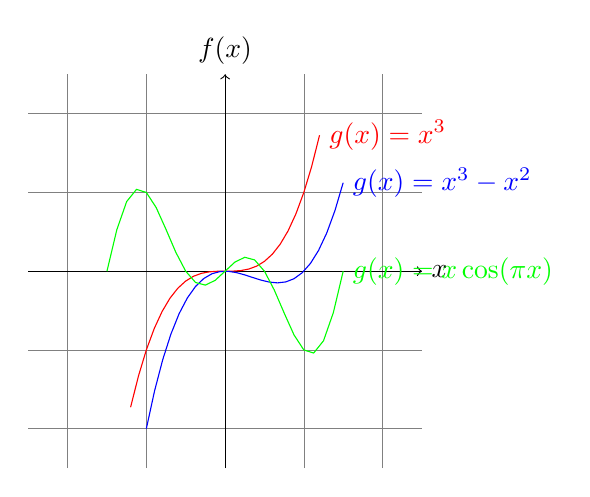
\begin{tikzpicture}
            \draw[very thin,color=gray] (-2.5, -2.5) grid (2.5, 2.5);
            \draw[->] (-2.5,0) -- (2.5,0) node[right] {$x$};
            \draw[->] (0,-2.5) -- (0,2.5) node[above] {$f(x)$};
            \draw[red,domain=-1.2:1.2]	plot (\x, { \x * \x * \x })   	node[right] {$g(x) = x^3 $};
            \draw[blue,domain=-1.0:1.5]	plot (\x, { \x * \x * \x - \x * \x })   	node[right] {$g(x) = x^3 - x^2$};
            \draw[green,domain=-1.5:1.5]	plot (\x, { \x * cos(3.1415926 * \x r) })   	node[right] {$g(x) = x\cos(\pi x) $};
        \end{tikzpicture}
    \end{minipage}
    \begin{minipage}[b]{0.32\textwidth}
        \centering
        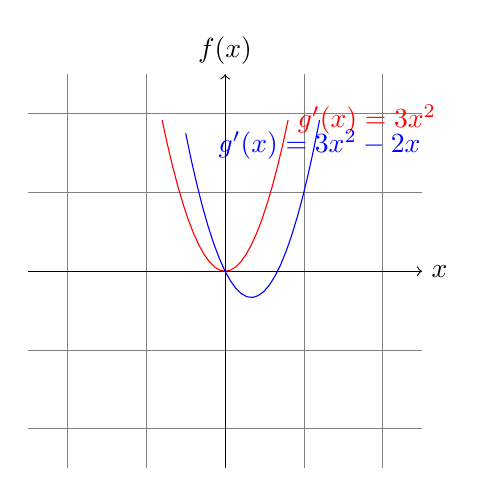
\begin{tikzpicture}
            \draw[very thin,color=gray] (-2.5, -2.5) grid (2.5, 2.5);
            \draw[->] (-2.5,0) -- (2.5,0) node[right] {$x$};
            \draw[->] (0,-2.5) -- (0,2.5) node[above] {$f(x)$};
            \draw[red,domain=-0.8:0.8]	plot (\x, { 3 * \x * \x })   	node[right] {$g'(x) = 3x^2 $};
            \draw[blue,domain=-0.5:1.2]	plot (\x, { 3 * \x * \x - 2 * \x})   	node[below] {$g'(x) = 3x^2 - 2x$};
        \end{tikzpicture}
    \end{minipage}
    \begin{minipage}[b]{0.32\textwidth}
        \centering
        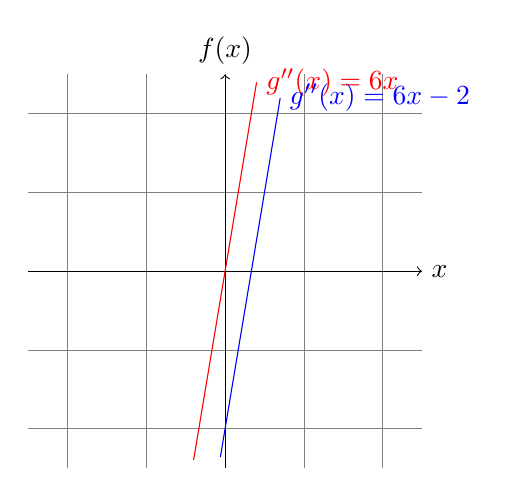
\begin{tikzpicture}
            \draw[very thin,color=gray] (-2.5, -2.5) grid (2.5, 2.5);
            \draw[->] (-2.5,0) -- (2.5,0) node[right] {$x$};
            \draw[->] (0,-2.5) -- (0,2.5) node[above] {$f(x)$};
            \draw[red,domain=-0.4:0.4]	plot (\x, { 6 * \x })   	node[right] {$g''(x) = 6x $};
            \draw[blue,domain=-0.06:0.7]	plot (\x, { 6 * \x - 2 })   	node[right] {$g''(x) = 6x - 2$};
        \end{tikzpicture}
    \end{minipage}
    \caption{Challenges}
\end{figure}


\subsection{Local Minima}
\begin{quotation}
    When the numerical solution of an optimization problem is near the local optimum, the numerical
    solution obtained by the final iteration may only minimize the objective function locally, rather
    than globally, as the gradient of the objective function's solutions approaches or becomes zero.
    \textit{Only some degree of noise might knock the parameter out of the local minimium. In fact,
        this is the one of the beneficial properties of stochastic gradient descent where the natural variation
        of gradients over minibatches is able to dislodge the parameters from loacl minima.}\cite{zhang2020dive}
\end{quotation}
\subsection{Saddle Points}
\begin{quotation}
    We assume that the input of a function is $k$-dimensional vector and its ouput is a scalar,
    so its \textit{Hession matrix} will have \textit{$k$ eigenvalues}. The solution of the function could
    be a local minimum, a local maximum or a saddle point at a position where the function gradient
    is zero:
    \begin{itemize}
        \item When the eigenvalues of the function's Hession matrix at the zero-gradient position
              are all positive, we have a local minimum for the function.
        \item When the eigenvalues of the function's Hession matrix at the zero-gradient position
              are all negative, we have a local maximum for the function.
        \item When the eigenvalues of the function's Hession matrix at the zero-gradient position
              are negative and positive, we have a saddle point for the function.
        \item 同号且至少有一个为0,不确定
    \end{itemize}
    For high-dimensional problem the likehood that at least some of the eigenvalues are negative
    is quite high. This makes sadlle points are more likely then local minima.\cite{zhang2020dive}
\end{quotation}

\subsection{Vanishing gradients}
\begin{quotation}
    Vanishing gradients can cause optimization to stall. Often a reparameterization of the problem
    helps. Good initialization of the parameters can be beneficial, too.\cite{zhang2020dive}
\end{quotation}

\subsection{noise / noise-free}
noise对优化过程中saddle point的影响?
what is nosie? and how it effect the optimization.
无偏估计、一致性

\section{Gradient Descent}
Using a Taylor expansion we obtain that:
\begin{equation}
    f(x + \epsilon) = f(x) + \epsilon f'(x) + \mathcal{O} (\epsilon^2)
\end{equation}
\par
For small $\epsilon$ moving in \textit{the direction of negative gradient} will decrease $f$. Choose $\epsilon =
    -\eta f'(x), \eta > 0$, then we get:
\begin{equation}
    f(x - \eta f'(x)) = f(x) - \eta f'^2(x) + \mathcal{O} ((\eta f'(x))^2)
\end{equation}
\par Choose $\eta$ samll enough for the higher order terms to become irrelevant. then
\begin{equation}
    f(x - \eta f'(x)) \lessapprox f(x)
\end{equation}
that means, if we use
\begin{equation}
    x \leftarrow x - \eta f'(x)
\end{equation}
to iterate x, the value of $f(x)$ decline.

\subsection{Adaptive Methods}
Getting the learning rate 'just right' is tricky. What if we could determine $\eta$ automatically or get rid of having to select
a setp size at all? Second order methods that look not only at the value and gradient of the objective but alse at its \textit{curvature}
can help in this case. These methods cannot be applied to deep learning directly due to the computational cost.

\subsubsection{Newton's Method}
当Taylor expansion展开到二阶导数时:
\begin{equation}
    f(\vx + \epsilon) = f(\vx) + \epsilon^\top \nabla f(\vx) + \frac{1}{2} \epsilon^\top H_f \epsilon
    + \mathcal{O}(\|\epsilon\|^3)
\end{equation}
we define $H_f := \nabla \nabla ^\top f(\vx)$ to be the \textit{Hession} of $f$. $H$ is a $d \times  d$ matrix and may be
prohibitively large, due to the cost of storing $\mathcal{O}(d^2)$ entries.

\par

After all, the minimum of $f$ statifies $\nabla f(\vx) = 0$.  Taking derivatives of above equtaion with regard to $\eta$ and
ignoring higher order terms we arrive at
\begin{equation}
    \begin{split}
        \nabla f(\vx) + H_f \epsilon = 0 \\
        \bm{\epsilon} = -H_f^{-1} \nabla f(\vx)
    \end{split}
\end{equation}

then, $\epsilon = -\eta \nabla f(\vx)$, we get
\begin{equation}
    \begin{split}
        \bm{\eta} = -H_f^{-1}
    \end{split}
\end{equation}

For $f(x) = (x-2)(x-4) = x^2 - 6x + 8, f'(x) = 2x - 6, f''(x) = 2$, then
\begin{equation}
    \epsilon = -f''(0)^{-1} f'(0) = -\frac{1}{2} \times -6 = 3
\end{equation}

\subsubsection{Hessian}
Hession 矩阵是是对称的,可以表示为一组特征值和一组特征向量的正交基底,在特定方向上$g$上的二阶导数为$g^\top H g$,当$g$为特征向量时,这个二阶导数就是
对应的特征值。最大特征值确定最大二阶导数,最小特征值确定最小导数。\par
在$g$方向上的learning rate为
\begin{equation}
    \eta_g = \frac{1}{g^\top H_f g}
\end{equation}
最差的情况下,$g$与$H$最大的特征值$\lambda_{max}$对应的特征向量对齐,此时的最优步长为$\frac{1}{\lambda_{max}}$,当要最小化的目标函数能用二次函数
很好近似的情况下,Hession的特征值决定了学习率的量级。

\subsection{Stochastic Gradient Descent}
\subsubsection{Dynamic Learning rate}

\begin{equation}
    \begin{aligned}
        \eta(t) & = \eta_i \text{ if } t_i \leq  t \leq t_{i+1} &  & piecewise constant \\
        \eta(t) & = \eta_0 e^{-\lambda t}                       &  & exponential        \\
        \eta(t) & = \eta_0 (\beta t + 1) ^{-\alpha}             &  & polynomial
    \end{aligned}
\end{equation}
In the case of convex optimization there are a number of proofs which show that this rate is well behaved.

\subsection{Minibatch Stochastic Gradient Descent}
At each iteration of stochastic gradient descent, we uniformly sample an index $i \in {i,..., n}$ for data examples at
random, and compute the gradient $\nabla f_i(\vx)$ to update $\vx$:
\begin{equation}
    \vx \leftarrow \vx - \eta \nabla f_i(\vx)
\end{equation}

The stochastic gradient $\nabla f_i(\vx)$ is the \textit{unbiased estimate} of gradient $\nabla f(\vx)$.
That means the stochastic gradient is a good estimate of the gradient.
\begin{equation}
    \E_i \nabla f_i(\vx) = \frac{1}{n} \sum_{i=1}^n \nabla f_i (\vx) = \nabla f(\vx)
\end{equation}

\section{SGDM - SGD with Momentum}

\begin{equation}
    \begin{split}
        \vv_t &\leftarrow \beta \vv_{t-1} + \nabla f(\vx) \\
        \vx_t &\leftarrow \vx_{t-1} - \eta_t \vv_{t}
    \end{split}
\end{equation}

$\vv$ is called \textit{momentum}. Momentum replaces gradients with a leaky average over past gradients. This
accelerates convergence significantly. And it prevents stalling of the optimization process that is much more
likely to occur for stochastic gradient descent.

\subsubsection{An Ill-conditioned Problem}
\begin{equation}
    f(\vx) = 0.1 x_1^2 + 2 x_2^2
\end{equation}
and we know that $f$ has minimum at $(0, 0)$. Then we get
\begin{equation}
    \nabla f(\vx) =
    \begin{bmatrix}
        0.2x_1 \\
        4x_2
    \end{bmatrix}
\end{equation}
let's start at $(2, 2)$, $\eta = 0.4, \beta = 0.6$.

\section{NAG - Nesterov Accelerated Gradient}
\begin{equation}
    \begin{split}
        \vv_t &= \alpha \vv_{t-1} + \eta \nabla_\theta J(\theta - \alpha \vv_{t-1})\\
        \theta &= \theta - \vv_t
    \end{split}
\end{equation}

\section{Adagrad}
Consider a model training on spare features, i.e., features that occur only infrequently. Parameters associated with infrequent
features only receive meaningful updates whenever these features occur. And to get good accuracy we want to decrease the lr as well
keep on training, usually at a lr of $\mathcal{O}(t^{-\frac{1}{2}})$. we might end up in situation where the parameters from common
features converge rather quickly to their optimal values.

\begin{equation}
    \begin{split}
        \vg_t &= \partial _{\vw} l(y_t, f(\vx_t, \vw))\\
        \vs_t &= \vs_{t-1} + \vg_t^2 \\
        \vw_t &= \vw_{t-1} - \frac{\eta}{\sqrt{\vs_t + \epsilon}} \cdot \vg_t
    \end{split}
\end{equation}
learning rate不再简单的是时间的函数,而是和梯度相关,lr的减小速度和梯度正相关,每个维度都有自己的learning rate.
\begin{quote}
    \begin{itemize}
        \item It uses the magnitude of the gradient as a means of adjusting how quickly progress is achieved - coordinates with large gradients are compensated with a smaller learning rate.
        \item On deep learning problems Adagrad can sometimes be too aggressive in reducing learning rates
    \end{itemize}
\end{quote}


\section{RMSProp}
A variant of AdaGrad.

\begin{quotation}
    As a result $\vs_t$ keeps on growing without bound due to the lack of normalization, essentially linearly
    as the algorithm converges.
\end{quotation}
\begin{equation}
    \begin{split}
        \vs_t &\leftarrow \gamma\vs_{t-1} + (1-\gamma)\vg^2_{t} \\
        \vx_t &\leftarrow \vx_{t-1} - \frac{\eta}{\sqrt{\vs_t + \epsilon}} \odot \vg_t
    \end{split}
\end{equation}

\begin{equation}
    \begin{split}
        \vs_t &= (1-\gamma) \vg^2_t + \gamma\vs_{t-1} \\
        &= (1-\gamma)(\vg^2_t + \gamma\vg^2_{t-1} + \gamma^2\vg^2_{t-2}+...)
    \end{split}
\end{equation}

\section{Adadelta}
A variant of AdaGrad.
\begin{equation}
    \begin{split}
        \vs_t &= \rho \vs_{t-1} + (1-\rho)\vg^2_t \\
        \vg'_t &= \frac{\sqrt{\Delta \vx_{t-1} + \epsilon}}{\sqrt{\vs_t + \epsilon}} \odot \vg_t\\
        \Delta \vx_t &= \rho \Delta \vx_{t-1} + (1 - \rho)\vg'^2_t\\
        \vx_t &= \vx_{t-1} - \vg'_t
    \end{split}
\end{equation}

\section{Adam}
\begin{equation}
    \begin{split}
        \vv_t &\leftarrow \beta_1 \vv_{t-1} + (1-\beta_1)\vg_t \\
        \vs_t &\leftarrow \beta_2 \vs_{t-1} + (1-\beta_2)\vg^2_t
    \end{split}
\end{equation}
Common choices for them are $\beta_1 = 0.9$ and $\beta_2 = 0.9999$. That is, the variance estimate moves \textit{much more slowly}
than the momentum term. Note that if we initialize $\vv_0 = \vs_0 = 0$ we have a significant amount of bias initally
towards smaller values. This can be addressed by using the fact that $\sum_{i=0}^t = \frac{1-\beta^t}{1-\beta}$ to re-normalize terms.
\begin{equation}
    \begin{split}
        \hat{\vv}_t &= \frac{\vv_t}{1-\beta_1^t} \\
        \hat{\vs}_t &= \frac{\vs_t}{1-\beta_2^t} \\
        \vx_t &\leftarrow \vx_{t-1} - \frac{\eta \hat{\vv}_t}{\sqrt{\hat{\vs}_t} + \epsilon}
    \end{split}
\end{equation}

\section{AdaMax}
\section{Nadam}
\section{AMSGrad}
